\documentclass{article}
\usepackage[utf8]{inputenc}
\usepackage[a4paper, total={7in, 10in}]{geometry}
\usepackage{libreriaLatex/float/float}
\usepackage{graphicx}
\usepackage{libreriaLatex/subfigure/subfigure}

\title{Métodos Computacionales - Tarea 4}
\author{Jesica Vanessa Caceres Naranjo - 201511555}
\date{Noviembre 2018}

\begin{document}

\maketitle
p
\section*{ODE - Movimiento de un proyectil}

Movimiento de un proyectil que sigue la ecuación

\begin{equation}
    \frac{d^{2}\vec{x}(t)}{dt^{2}}=-\vec{g}-c\frac{|\vec{x}(t)|^{2}}{m}\frac{\vec{x}(t)}{|\vec{x}(t)|}
\end{equation}

A continuación se observa el comportamiento del proyectil para unas condiciones iniciales:

\begin{equation}
    \vec{x}(t=0)=(0,0) \qquad \vec{v}(t=0)=300(cos(\phi),sin(\phi))
\end{equation}

\begin{figure}[H]
    \centering
    \subfigure[]{\label{fig:proyectilAngulo45}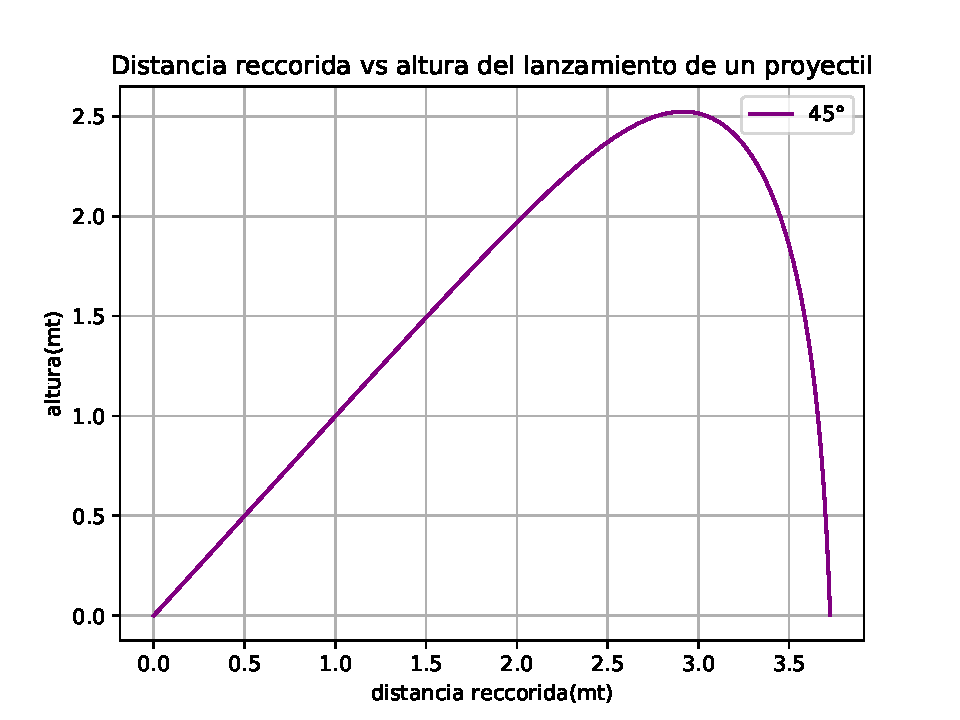
\includegraphics[scale = 0.4]{45.pdf}}
    \subfigure[]{\label{fig:proyectilDiferentesAngulos}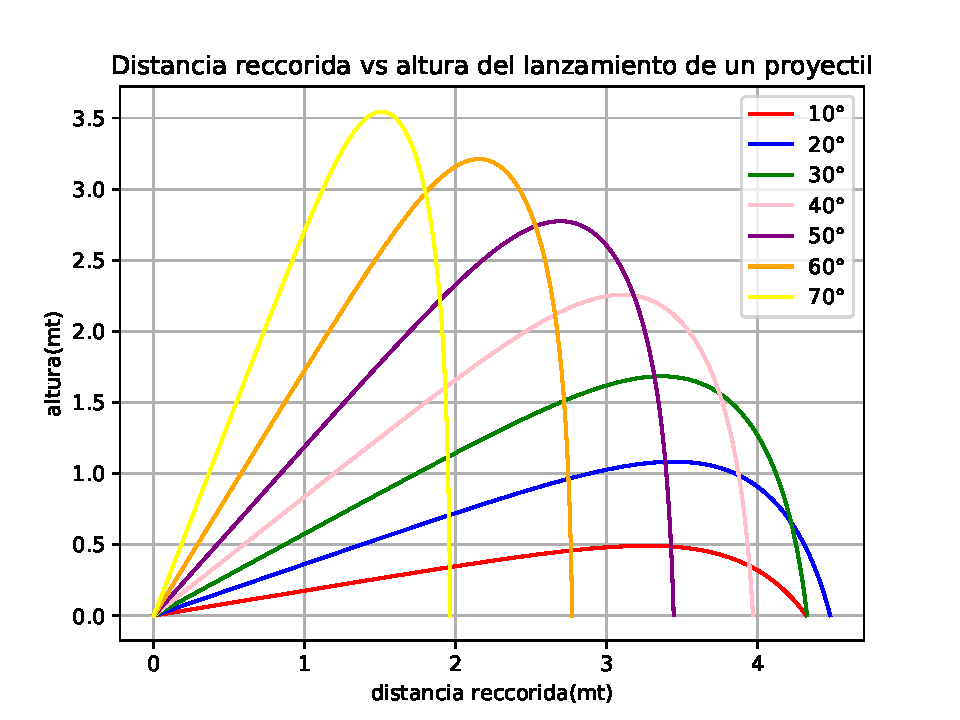
\includegraphics[scale = 0.4]{OtrosAngulos.pdf}}
    \caption{Movimiento de un proyectil en los planos X y Y para una velocidad inicial V0 con ángulo $\phi$ igual a a) 45$^{\circ}$ y b) (10-70)$^{\circ}$}
    \label{fig:CondicionesFijasTemp}
\end{figure}

Para la gráfica de 45 grados (Punto 1), se obtuvo que la distancia recorrida es: 3.72618m

Para la segunda gráfica (Punto 2), se obtuvo que la distancia máxima recorrida es: 4.48144m y se da para un ángulo de 20 grados.


\section*{PDE - Temperatura en una roca de calcita}

Comportamiento de la temperatura en una sección 2D de 50x50cm de una roca de calcita con una varilla cilíndrica incrustada perpendicularmente de diámetro 10cm. Aquí, la ecuación que rige el comportamiento de la temperatura es:

\begin{equation}
    \frac{dT(x,y)}{dt}=\nu\frac{d^{2}T(x,y)}{dx^{2}}+\nu\frac{d^{2}T(x,y)}{dy^{2}}
\end{equation}

La varilla posee una temperatura de 100$^{\circ}C$ constantes. Las condiciones iniciales de temperatura para la roca de calcita es de 10$^{\circ}C$ y las condiciones de frontera se dan para diferentes casos. Para cada caso, se realizo una simulación para un tiempo de 1500, con un dt = 1.5s/N donde N es 80. En cada uno, se realizaron 5 cuatro gráficas, que constatan la evolución de la temperatura en diferentes puntos del tiempo. La primera hace referencia al estado inicial, la segunda al primer avance, la tercera al segundo avance, la cuarta a la configuración de equilibrio y la quinta al promedio. En cada una de las gráficas, el eje x y y están en unidades de metros, entre 0-0.5m que es el tamaño de la placa de calcita y el eje z, está en unidades de kelvin (Kº)

Para cada grafica, los ejes X y Y (plano inferior) representan una sección 2D de la calcita con la varilla, en unidades de metros [m]. En el eje Z, se evidencia una superficie que representa la temperatura de la muestra en ese punto (X,Y), estando esta temperatura en Kelvin [K]. 

\subsection*{Condiciones de frontera fijas}

Las fronteras se mantienen a 10$^{\circ}C$ para toda la simulación ya que sus fronteras son fijas.
\begin{figure}[H]
    \centering
    \subfigure[]{\label{fig:temperaturaCondFi1}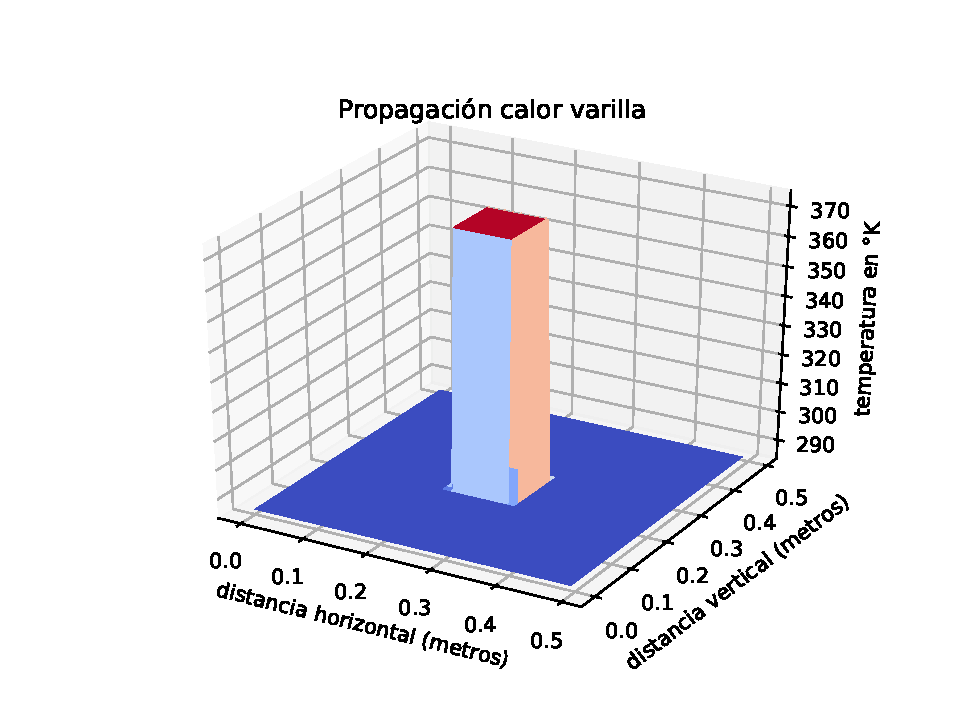
\includegraphics[scale = 0.3]{FronterasFijasInicial.pdf}}
    \subfigure[]{\label{fig:temperaturaCondFi2}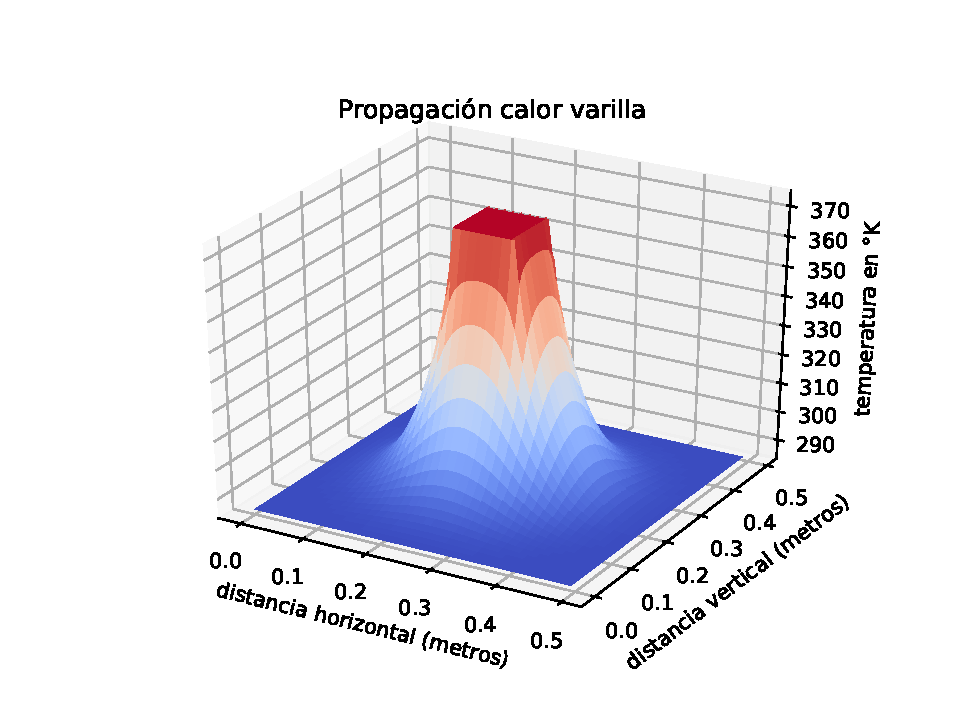
\includegraphics[scale = 0.3]{FronterasFijasAvance1.pdf}}
    \subfigure[]{\label{fig:temperaturaCondFi3}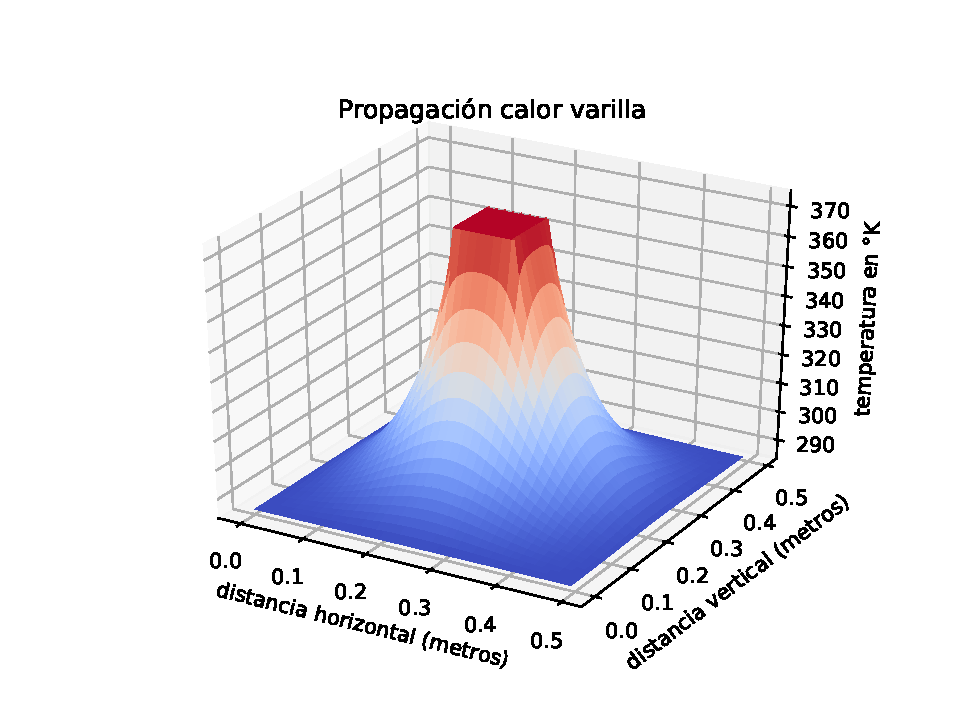
\includegraphics[scale = 0.3]{FronterasFijasAvance2.pdf}}
    \subfigure[]{\label{fig:temperaturaCondFi4}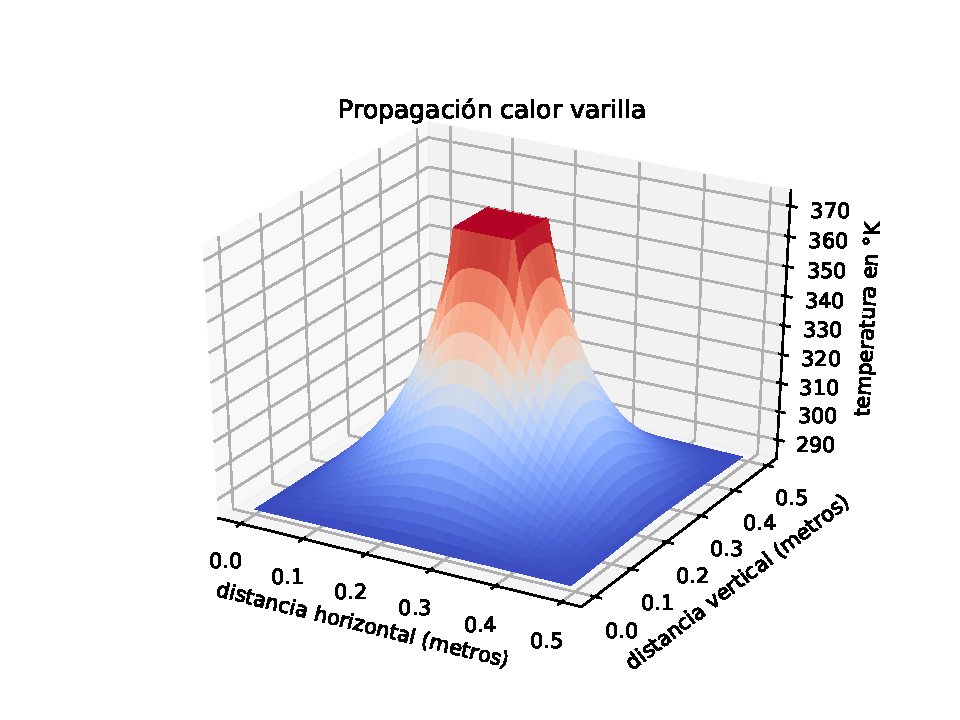
\includegraphics[scale = 0.3]{FronterasFijasEq.pdf}}
    \subfigure[]{\label{fig:temperaturaCondFi4}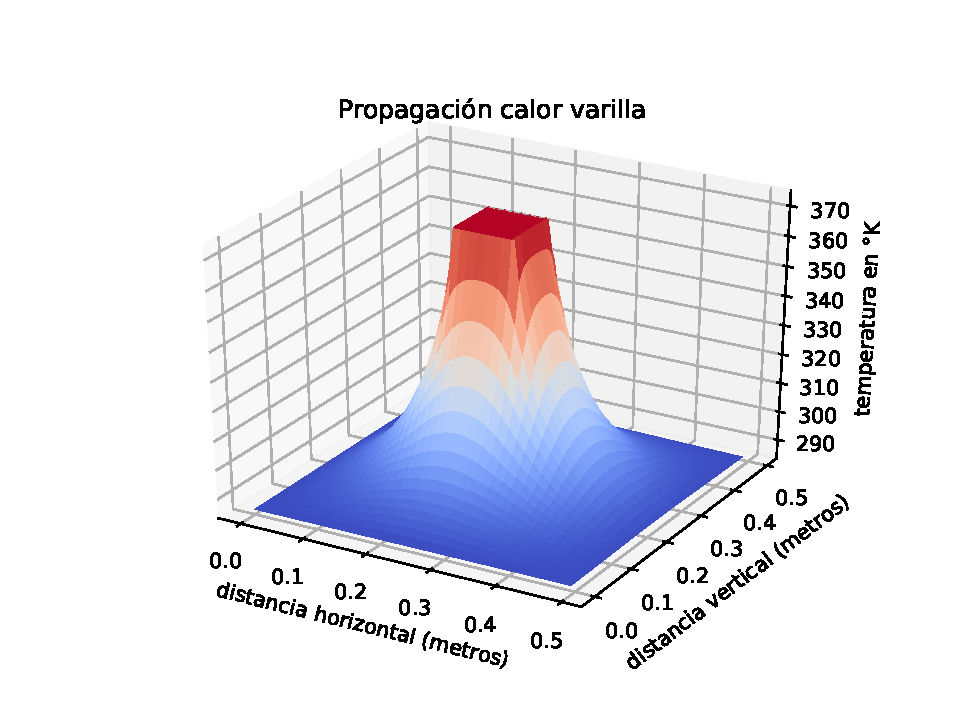
\includegraphics[scale = 0.3]{FronterasFijasPromedio.pdf}}
    \caption{Diagrama de temperatura de una placa metálica con una barra en la mitad con condiciones fijas para un tiempo a) En el tiempo 0 (t = 0), b) Avance 1 (t = t/3), c) avance 2(t = 2t/3), d) Equilibrio(t = T), e) Promedio.}
    \label{fig:CondicionesFijasTemp}
\end{figure}
\subsection*{Condiciones de frontera abiertas}
Las fronteras se mantienen libres para toda la simulación. En este caso, se observa que que las fronteras empiezan gradualmente a aumentar su temperatura.
\begin{figure}[H]
    \centering
    \subfigure[]{\label{fig:temperaturaCondAb1}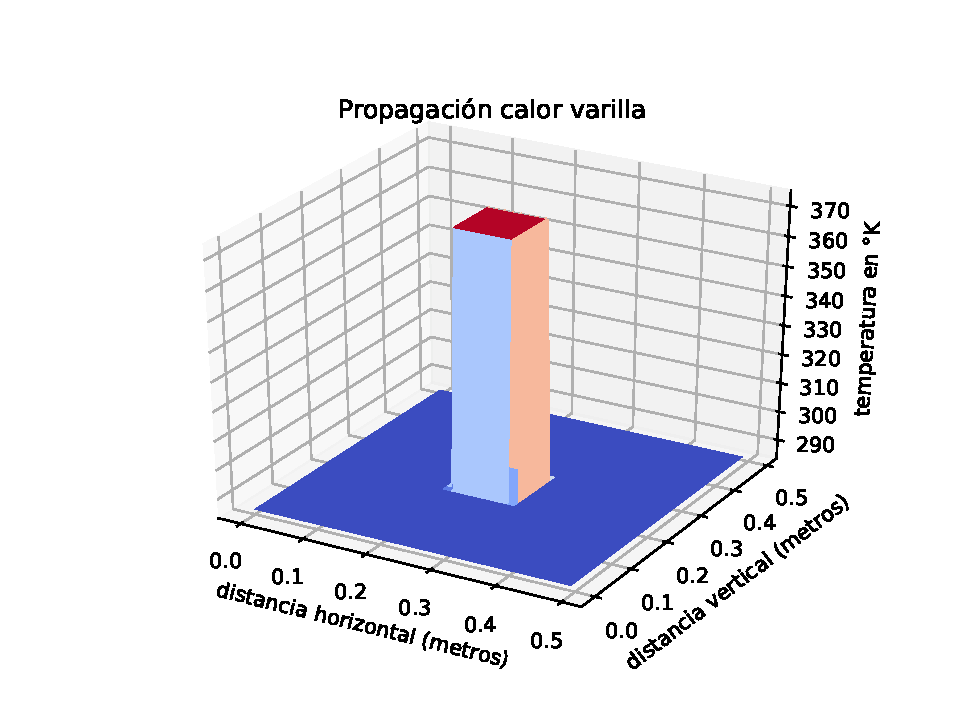
\includegraphics[scale = 0.3]{FronterasAbiertasInicial.pdf}}
    \subfigure[]{\label{fig:temperaturaCondAb2}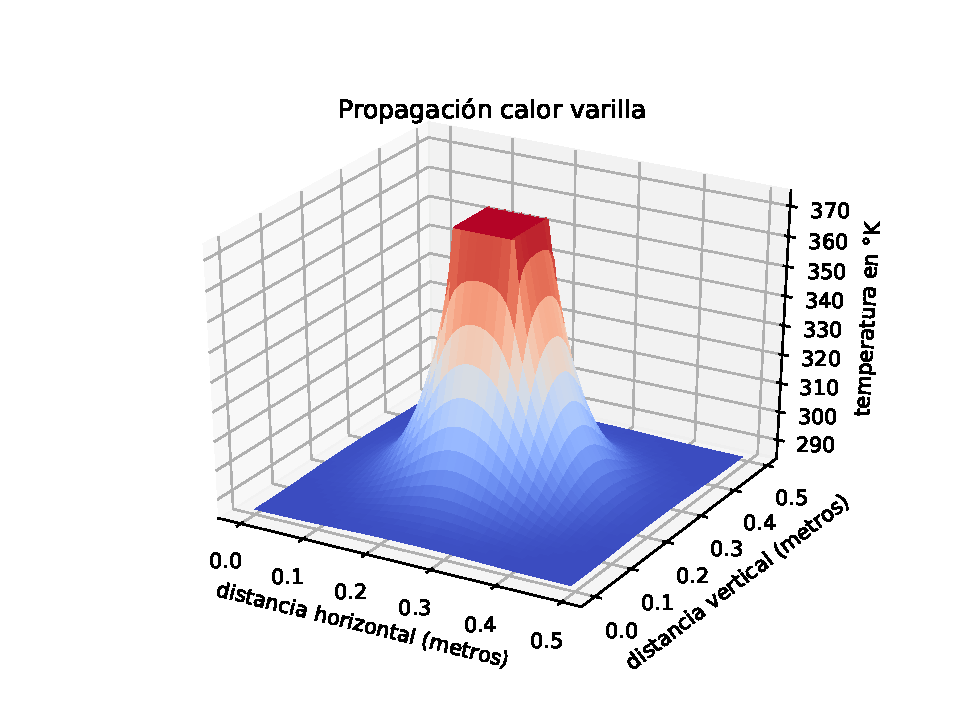
\includegraphics[scale = 0.3]{FronterasAbiertasAvance1.pdf}}
    \subfigure[]{\label{fig:temperaturaCondAb3}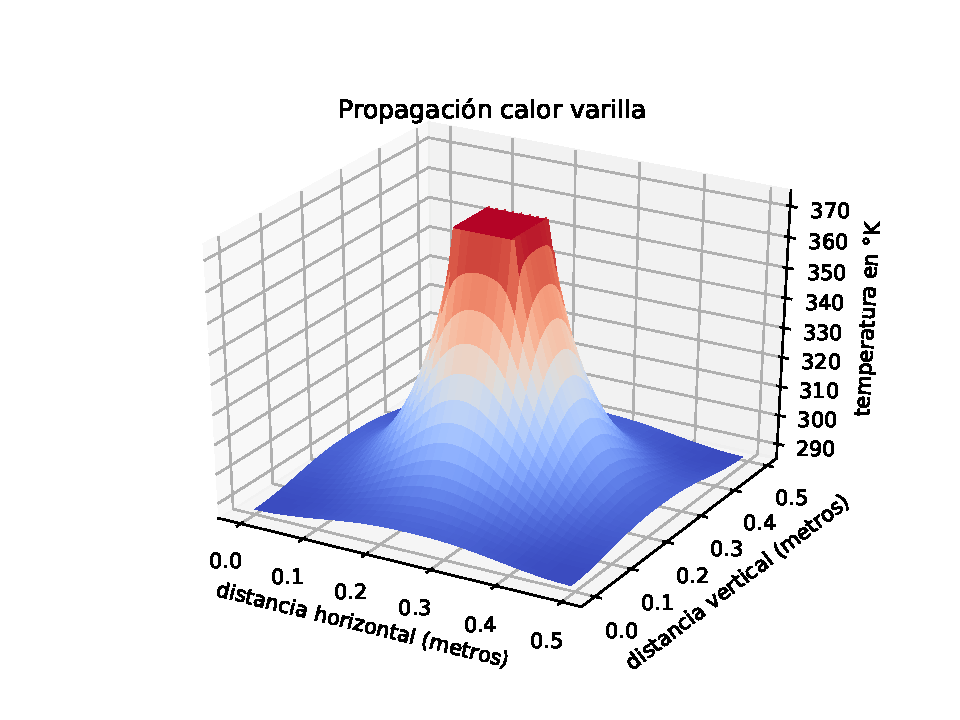
\includegraphics[scale = 0.3]{FronterasAbiertasAvance2.pdf}}
    \subfigure[]{\label{fig:temperaturaCondAb4}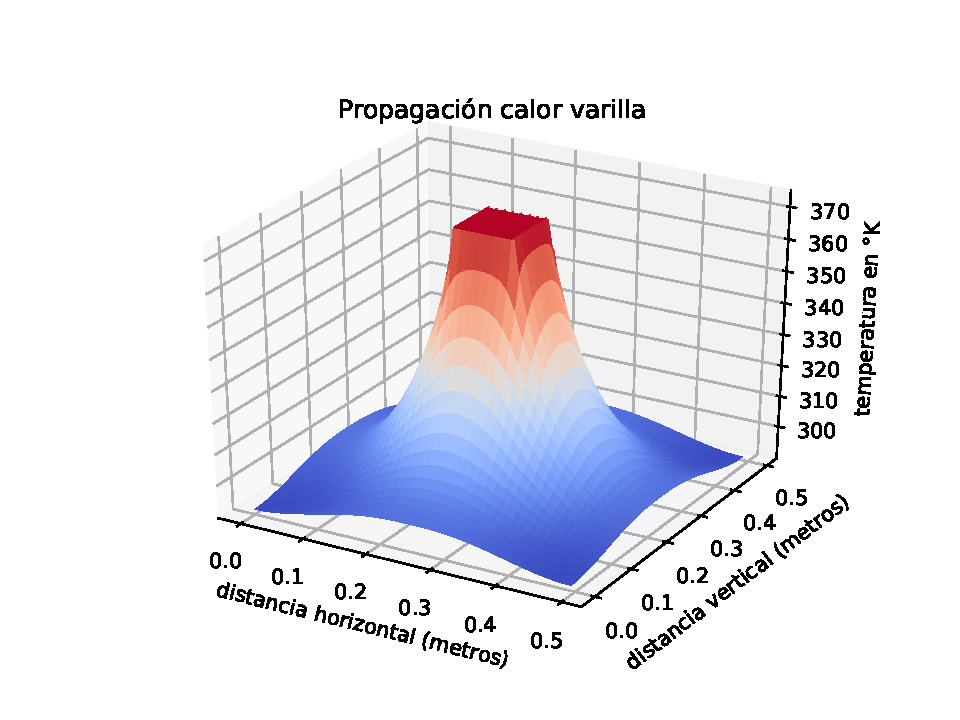
\includegraphics[scale = 0.3]{FronterasAbiertasEq.pdf}}
    \subfigure[]{\label{fig:temperaturaCondAb4}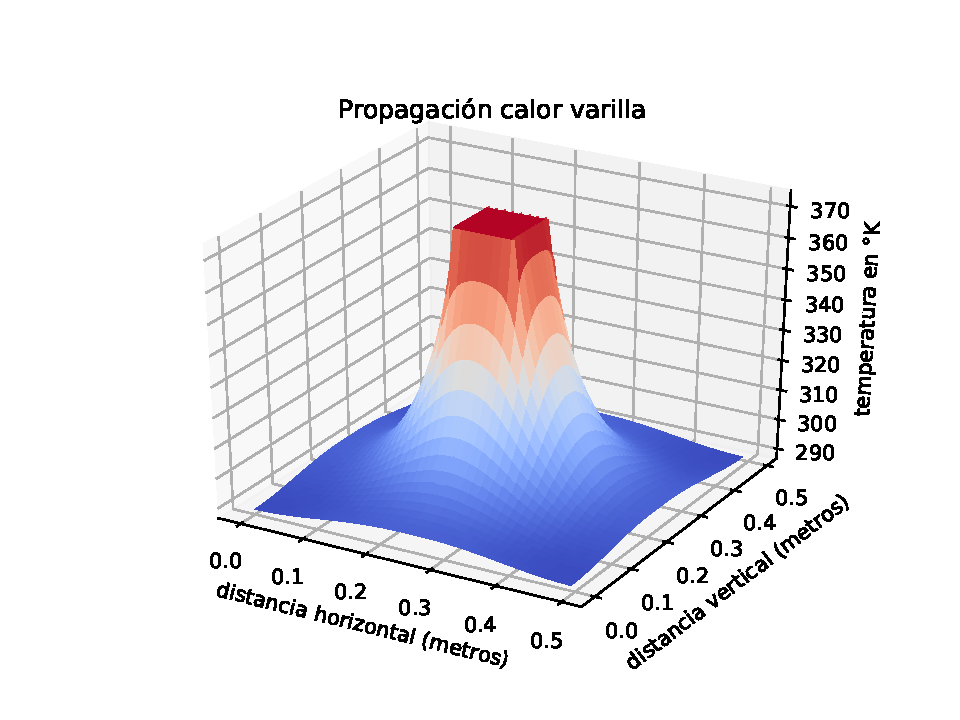
\includegraphics[scale = 0.3]{FronterasAbiertasPromedio.pdf}}
    \caption{Diagrama de temperatura de una placa metálica con una barra cilíndrica en la mitad con condiciones abiertas para un tiempo a) En el tiempo 0 (t = 0), b) Avance 1 (t = t/3), c) avance 2(t = 2t/3), d) Equilibrio(t = T), e) Promedio.}
    \label{fig:CondicionesFijasTemp}
\end{figure}
\subsection*{Condiciones de frontera periódicas}
Las fronteras se mantienen libres y periódicas para toda la simulación. En este caso, se observa que que las fronteras empiezan gradualmente a aumentar su temperatura y las  varilla a disminuir.
\begin{figure}[H]
    \centering
    \subfigure[]{\label{fig:temperaturaCondPe1}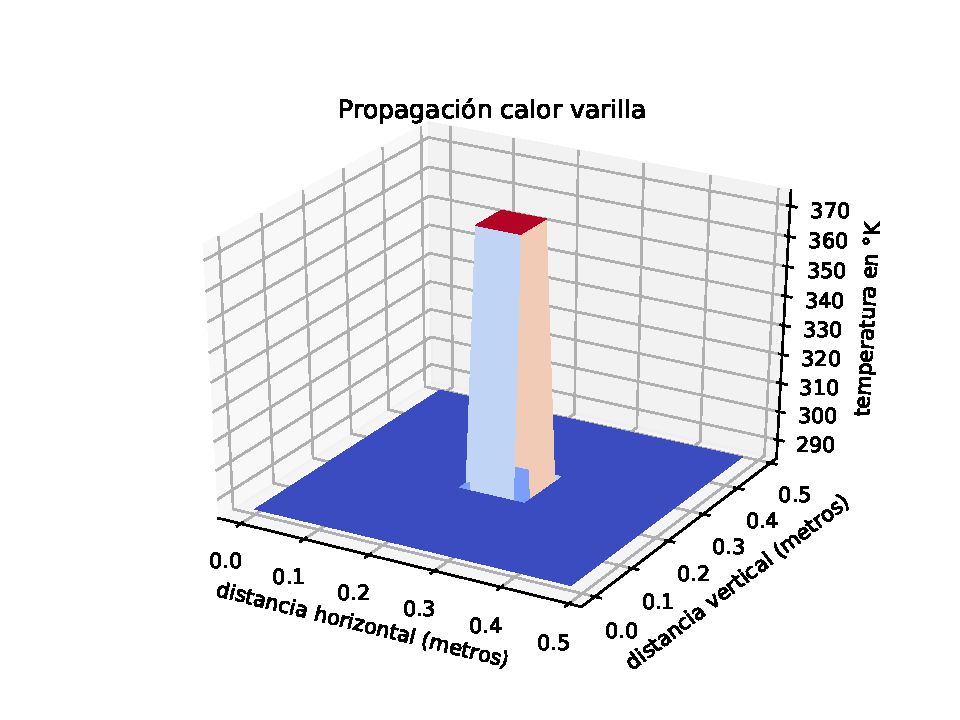
\includegraphics[scale = 0.3]{FronterasPeriodicasInicial.pdf}}
    \subfigure[]{\label{fig:temperaturaCondPe2}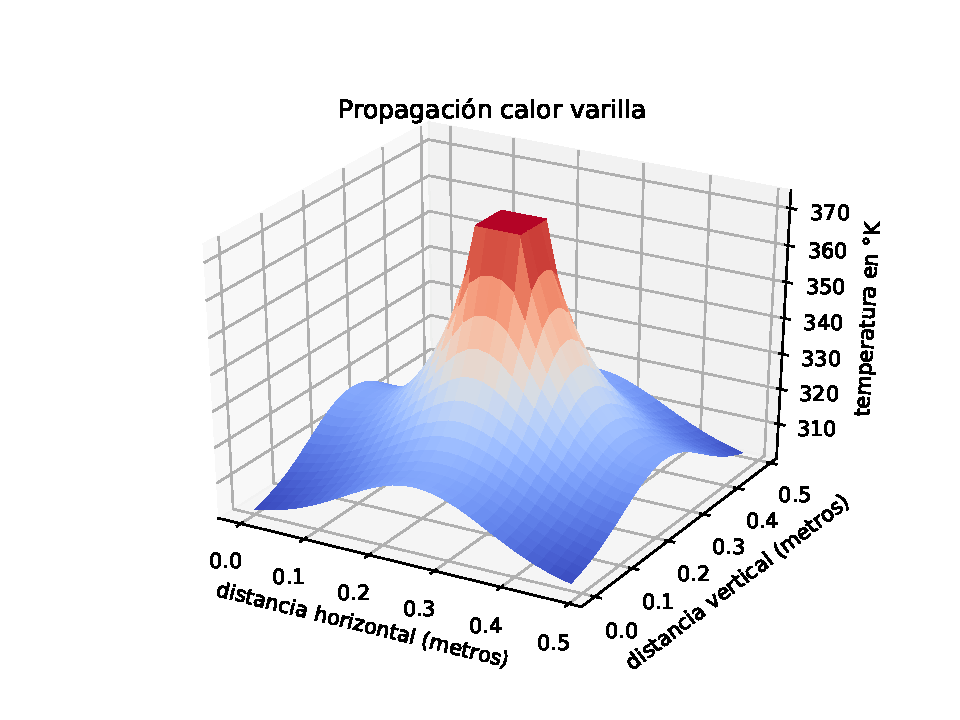
\includegraphics[scale = 0.3]{FronterasPeriodicasAvance1.pdf}}
    \subfigure[]{\label{fig:temperaturaCondPe3}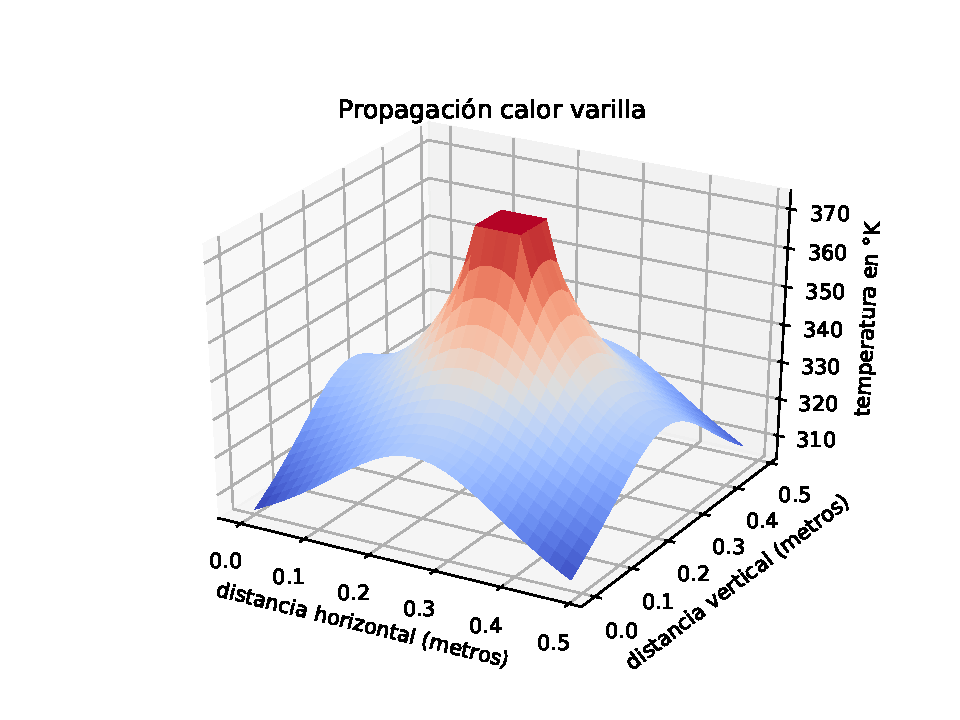
\includegraphics[scale = 0.3]{FronterasPeriodicasAvance2.pdf}}
    \subfigure[]{\label{fig:temperaturaCondPe4}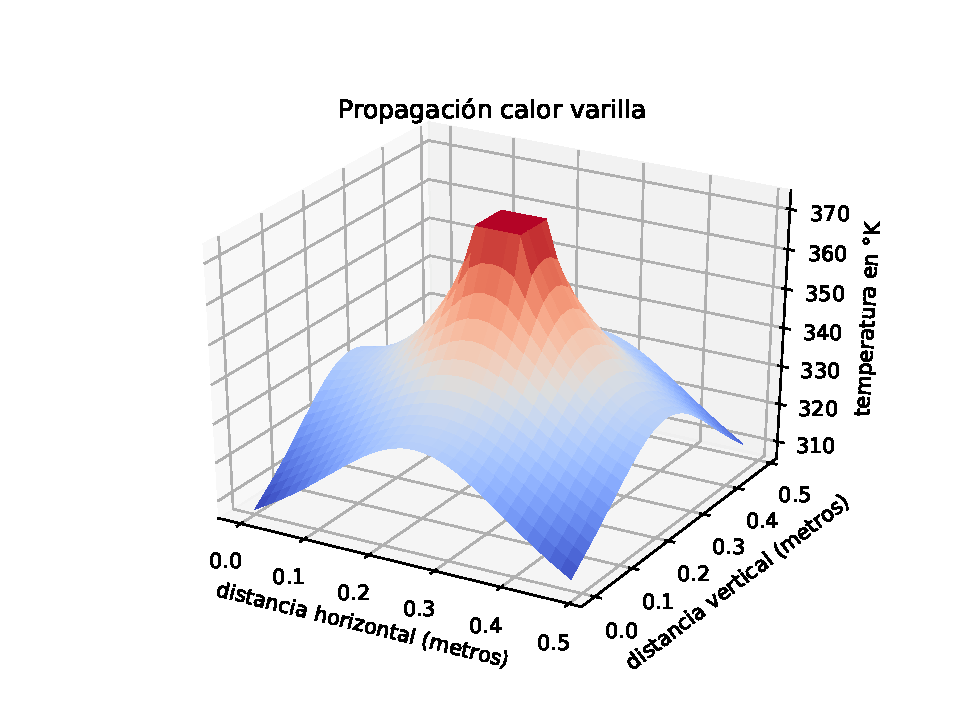
\includegraphics[scale = 0.3]{FronterasPeriodicasEq.pdf}}
    \subfigure[]{\label{fig:temperaturaCondPe4}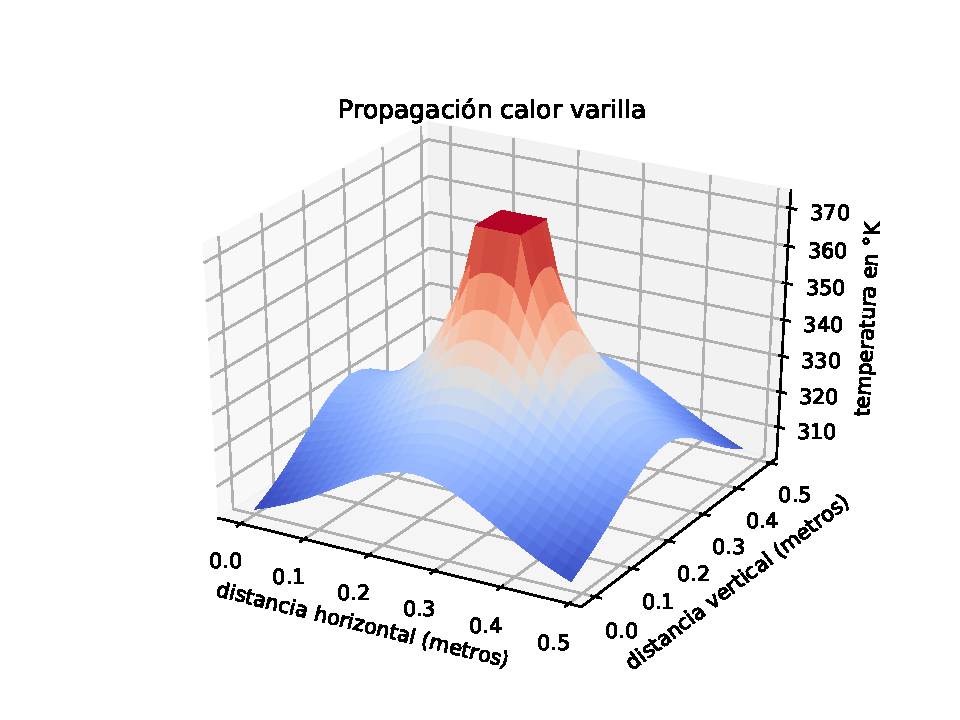
\includegraphics[scale = 0.3]{FronterasPeriodicasPromedio.pdf}}
    \caption{Diagrama de temperatura de una placa metálica con una barra cilíndrica en la mitad con condiciones periódicas para un tiempo a) En el tiempo 0 (t = 0), b) Avance 1 (t = t/3), c) avance 2(t = 2t/3), d) Equilibrio(t = T), e) Promedio.}
    \label{fig:CondicionesFijasTemp}
\end{figure}

\subsection*{Temperatura promedio en la calcita}
Para este caso, se obtuvieron los datos de la temperatura promedio en la calcita para cada caso de condiciones de frontera, y se graficó en el tiempo:

\begin{figure}[H]
    \centering
    \subfigure[]{\label{fig:temperaturaPromedioTiempo}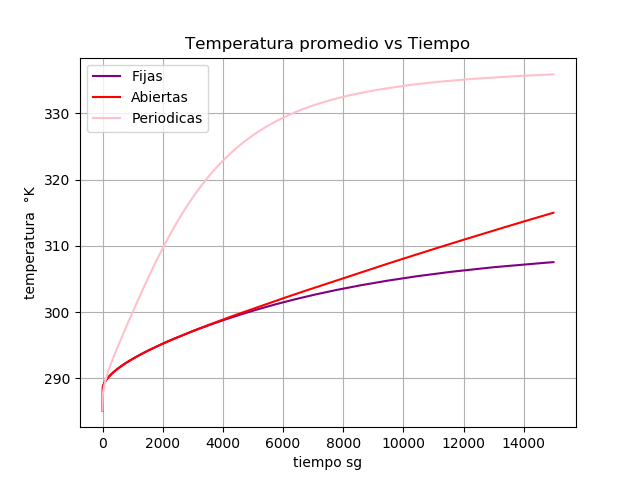
\includegraphics[scale = 0.4]{temperaturaPromedio.pdf}}
    \subfigure[]{\label{fig:temperaturaPromedioTiempoLog}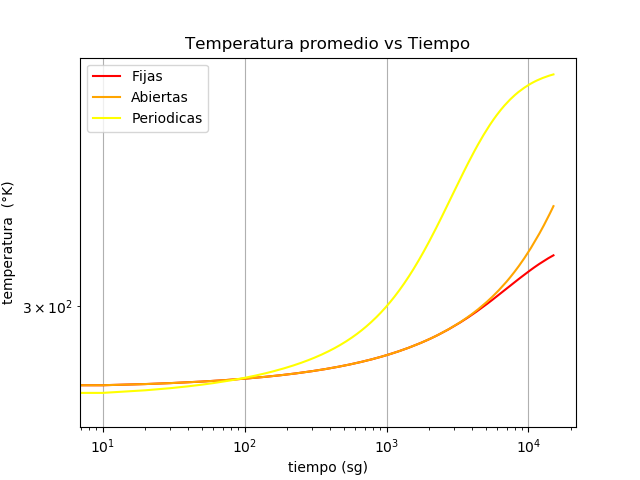
\includegraphics[scale = 0.4]{temperaturaPromedioLogarimtica.pdf}}
    \caption{Temperatura promedio en la calcita en función del tiempo para cada caso en escala a) lineal b) logaritmica.}
    \label{fig:CondicionesFijasTemp}
\end{figure}
\end{document}
